\section{Touch Sensor Arduino}
	\subsection{Penjelasan Sensor}
		Touch sensor adalah detektor panel sentuh yang memberikan satu tombol sentuh, ketika bantalan atau alas sensor disentuh, kapasitansi rangkaian akan berubah dan terdeteksi. Perubahan yang terdeteksi dalam kapasitansi, menghasilkan perubahan keadaan output.
		
		\begin{figure}[ht]
			\centerline{\includegraphics[width=0.5\textwidth]{figures/Depan.jpg}}
			\caption{Sensor Capacitive Bagian Depan}
			\label{Depan}
			\end{figure}
		Pada gambar \ref{Depan}  adalah merupakan gambar tampak depan pada touch sensor arduino kelompok kami.
		
		\begin{figure}[ht]
			\centerline{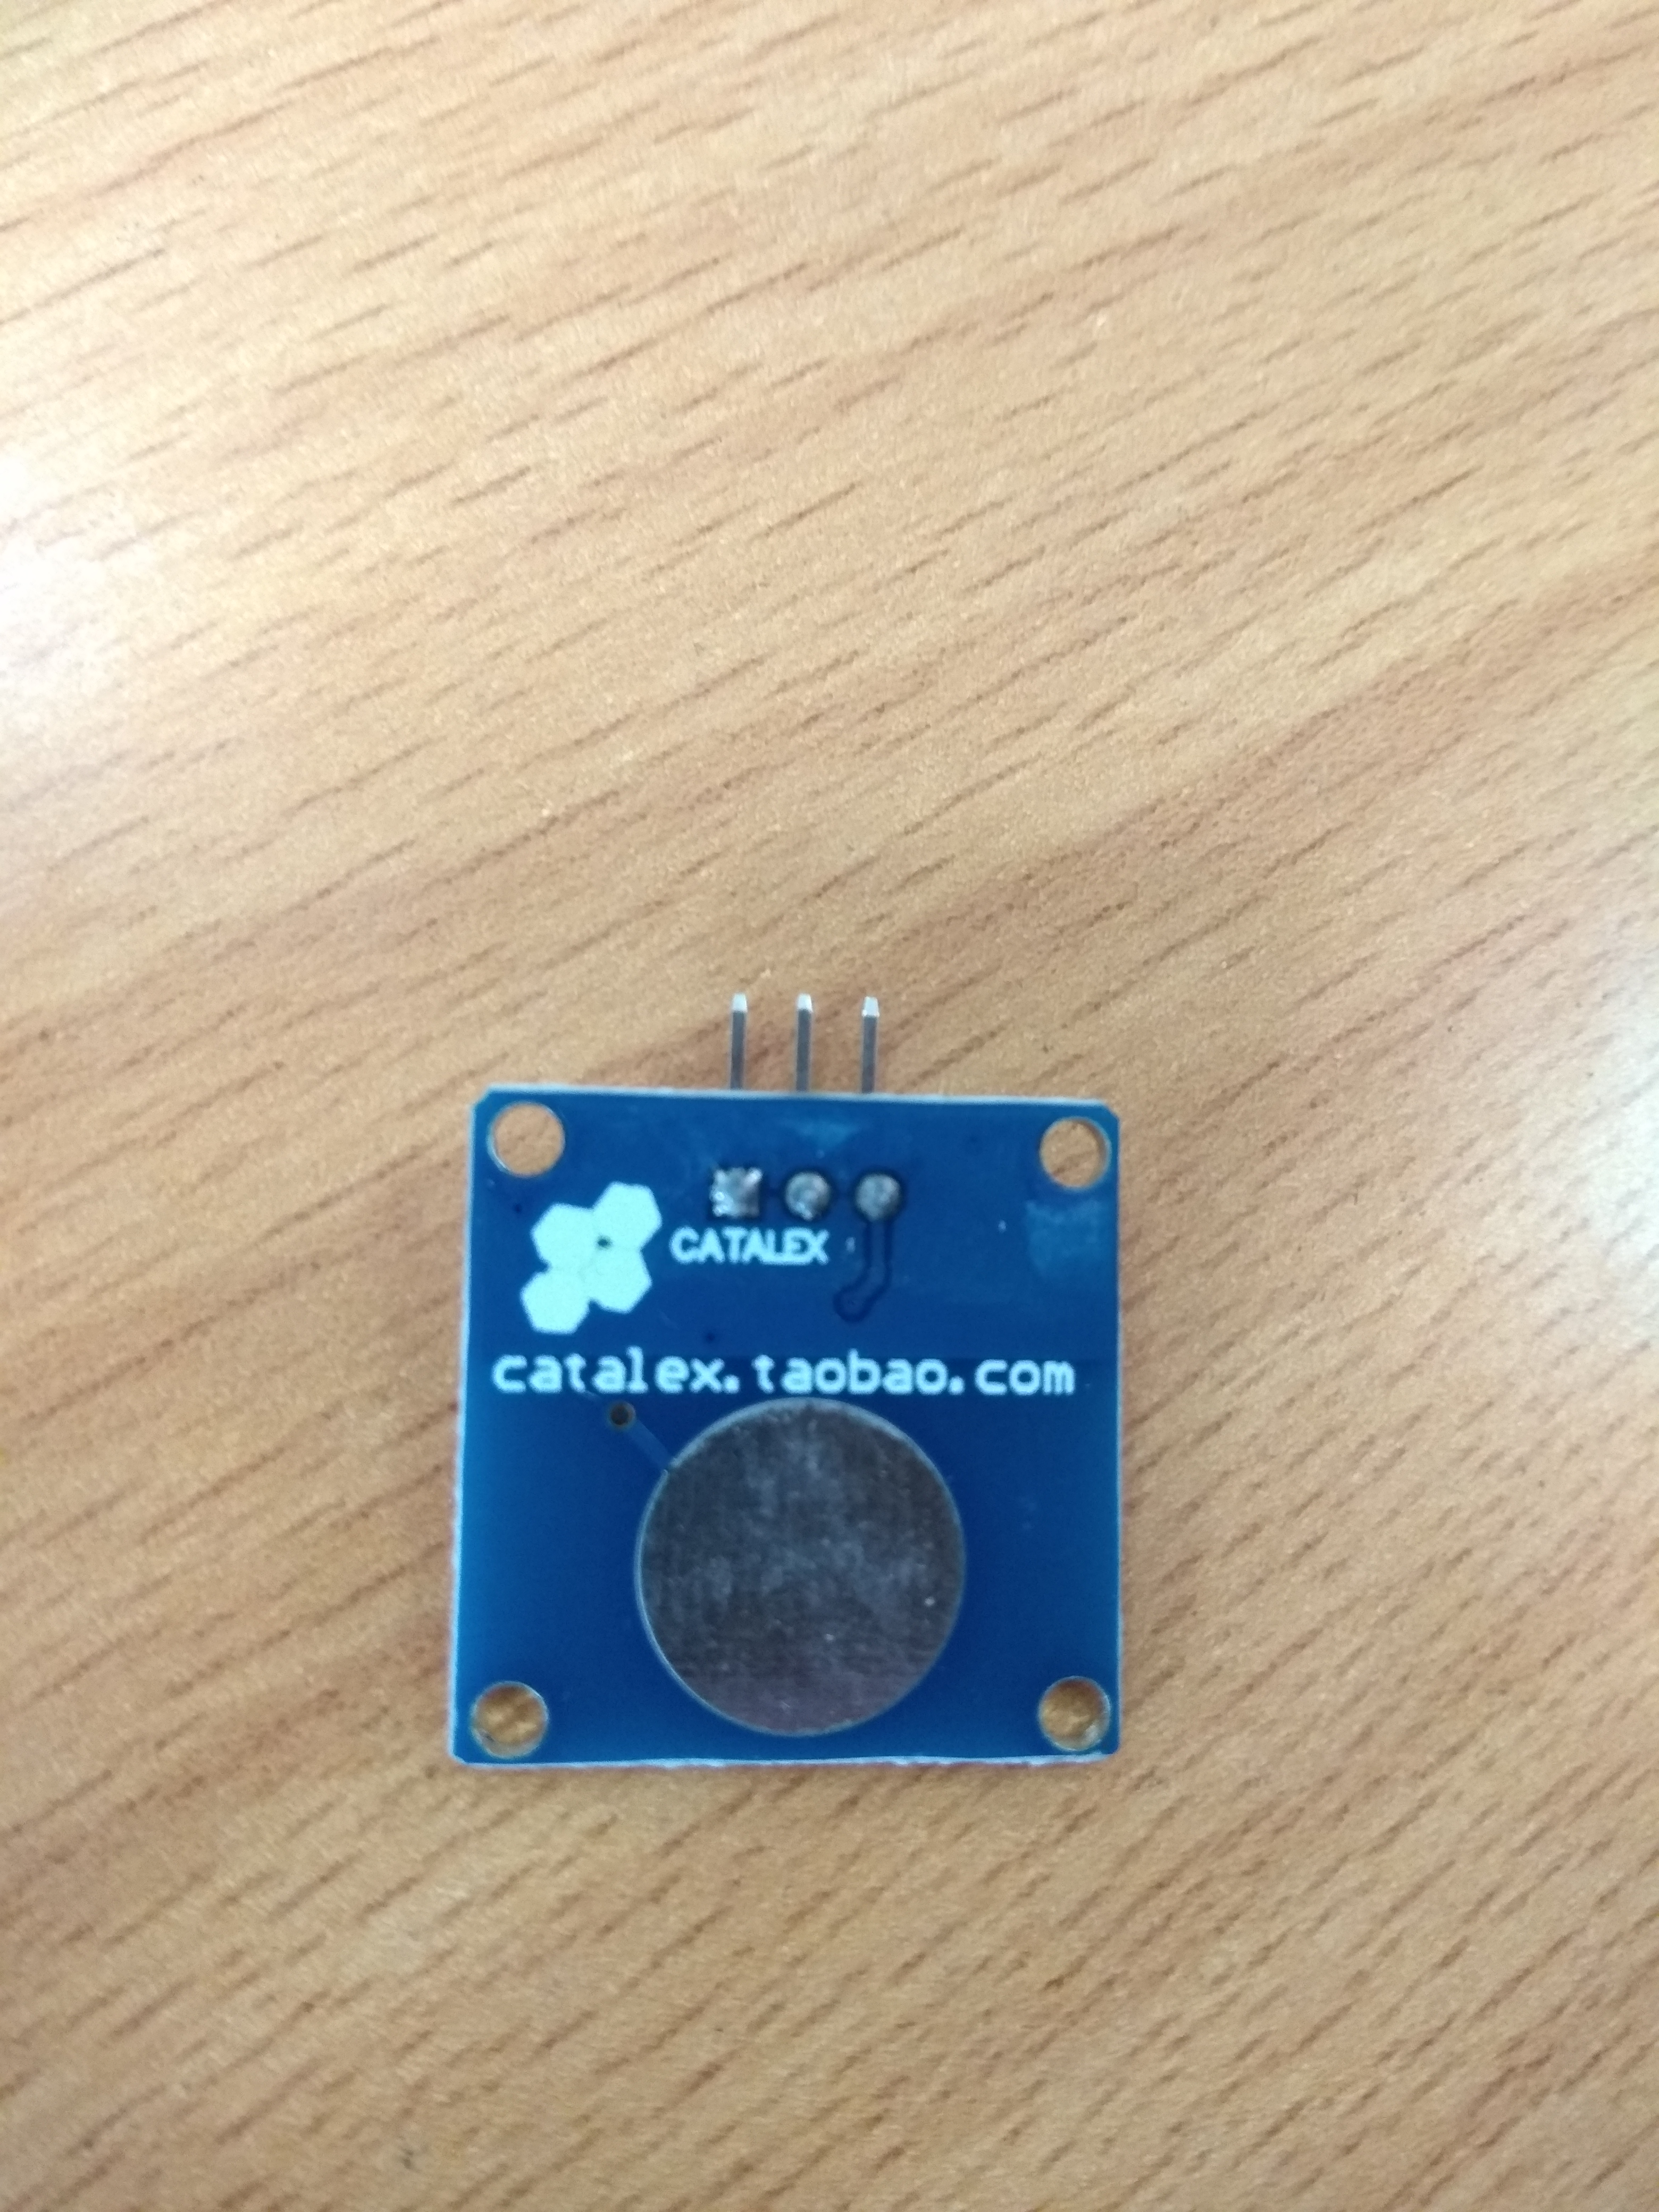
\includegraphics[width=0.5\textwidth]{figures/Belakang.jpg}}
			\caption{Sensor Capacitive Bagian Belakang}
			\label{Belakang}
			\end{figure}
		Pada Gambar \ref{Belakang} adalah merupakan gambar tampak belakang pada touch sensor arduino kelompok kami.
		
		
	\subsection{Kodingan}
	Berikut adalah coding pada sensor touch arduino kelompok kami :
	
	\begingroup\makeatletter\def\@currenvir{verbatim}
		\verbatim
		#define ctsPin 2 // Pin touch sensor
 
		int ledPin = 13; // pin the LED
 
		void setup() {
		  Serial.begin(9600);
		  pinMode(ledPin, OUTPUT);  
		  pinMode(ctsPin, INPUT);
		}
		 
		void loop() {
		  int ctsValue = digitalRead(ctsPin);
		  if (ctsValue == HIGH){
			digitalWrite(ledPin, HIGH);
			Serial.println("TOUCHED");
		  }
		  else{
			digitalWrite(ledPin,LOW);
			Serial.println("not touched");
		  } 
		  delay{500};
		  
		}
		\end{verbatim}
		
	\subsection{Hasil Projek}
		
		\begin{figure}[ht]
			\centerline{\includegraphics[width=0.5\textwidth]{figures/sebelum.jpg}}
			\caption{Sudah dirakit}
			\label{sebelum}
			\end{figure}
			
		\begin{figure}[ht]
			\centerline{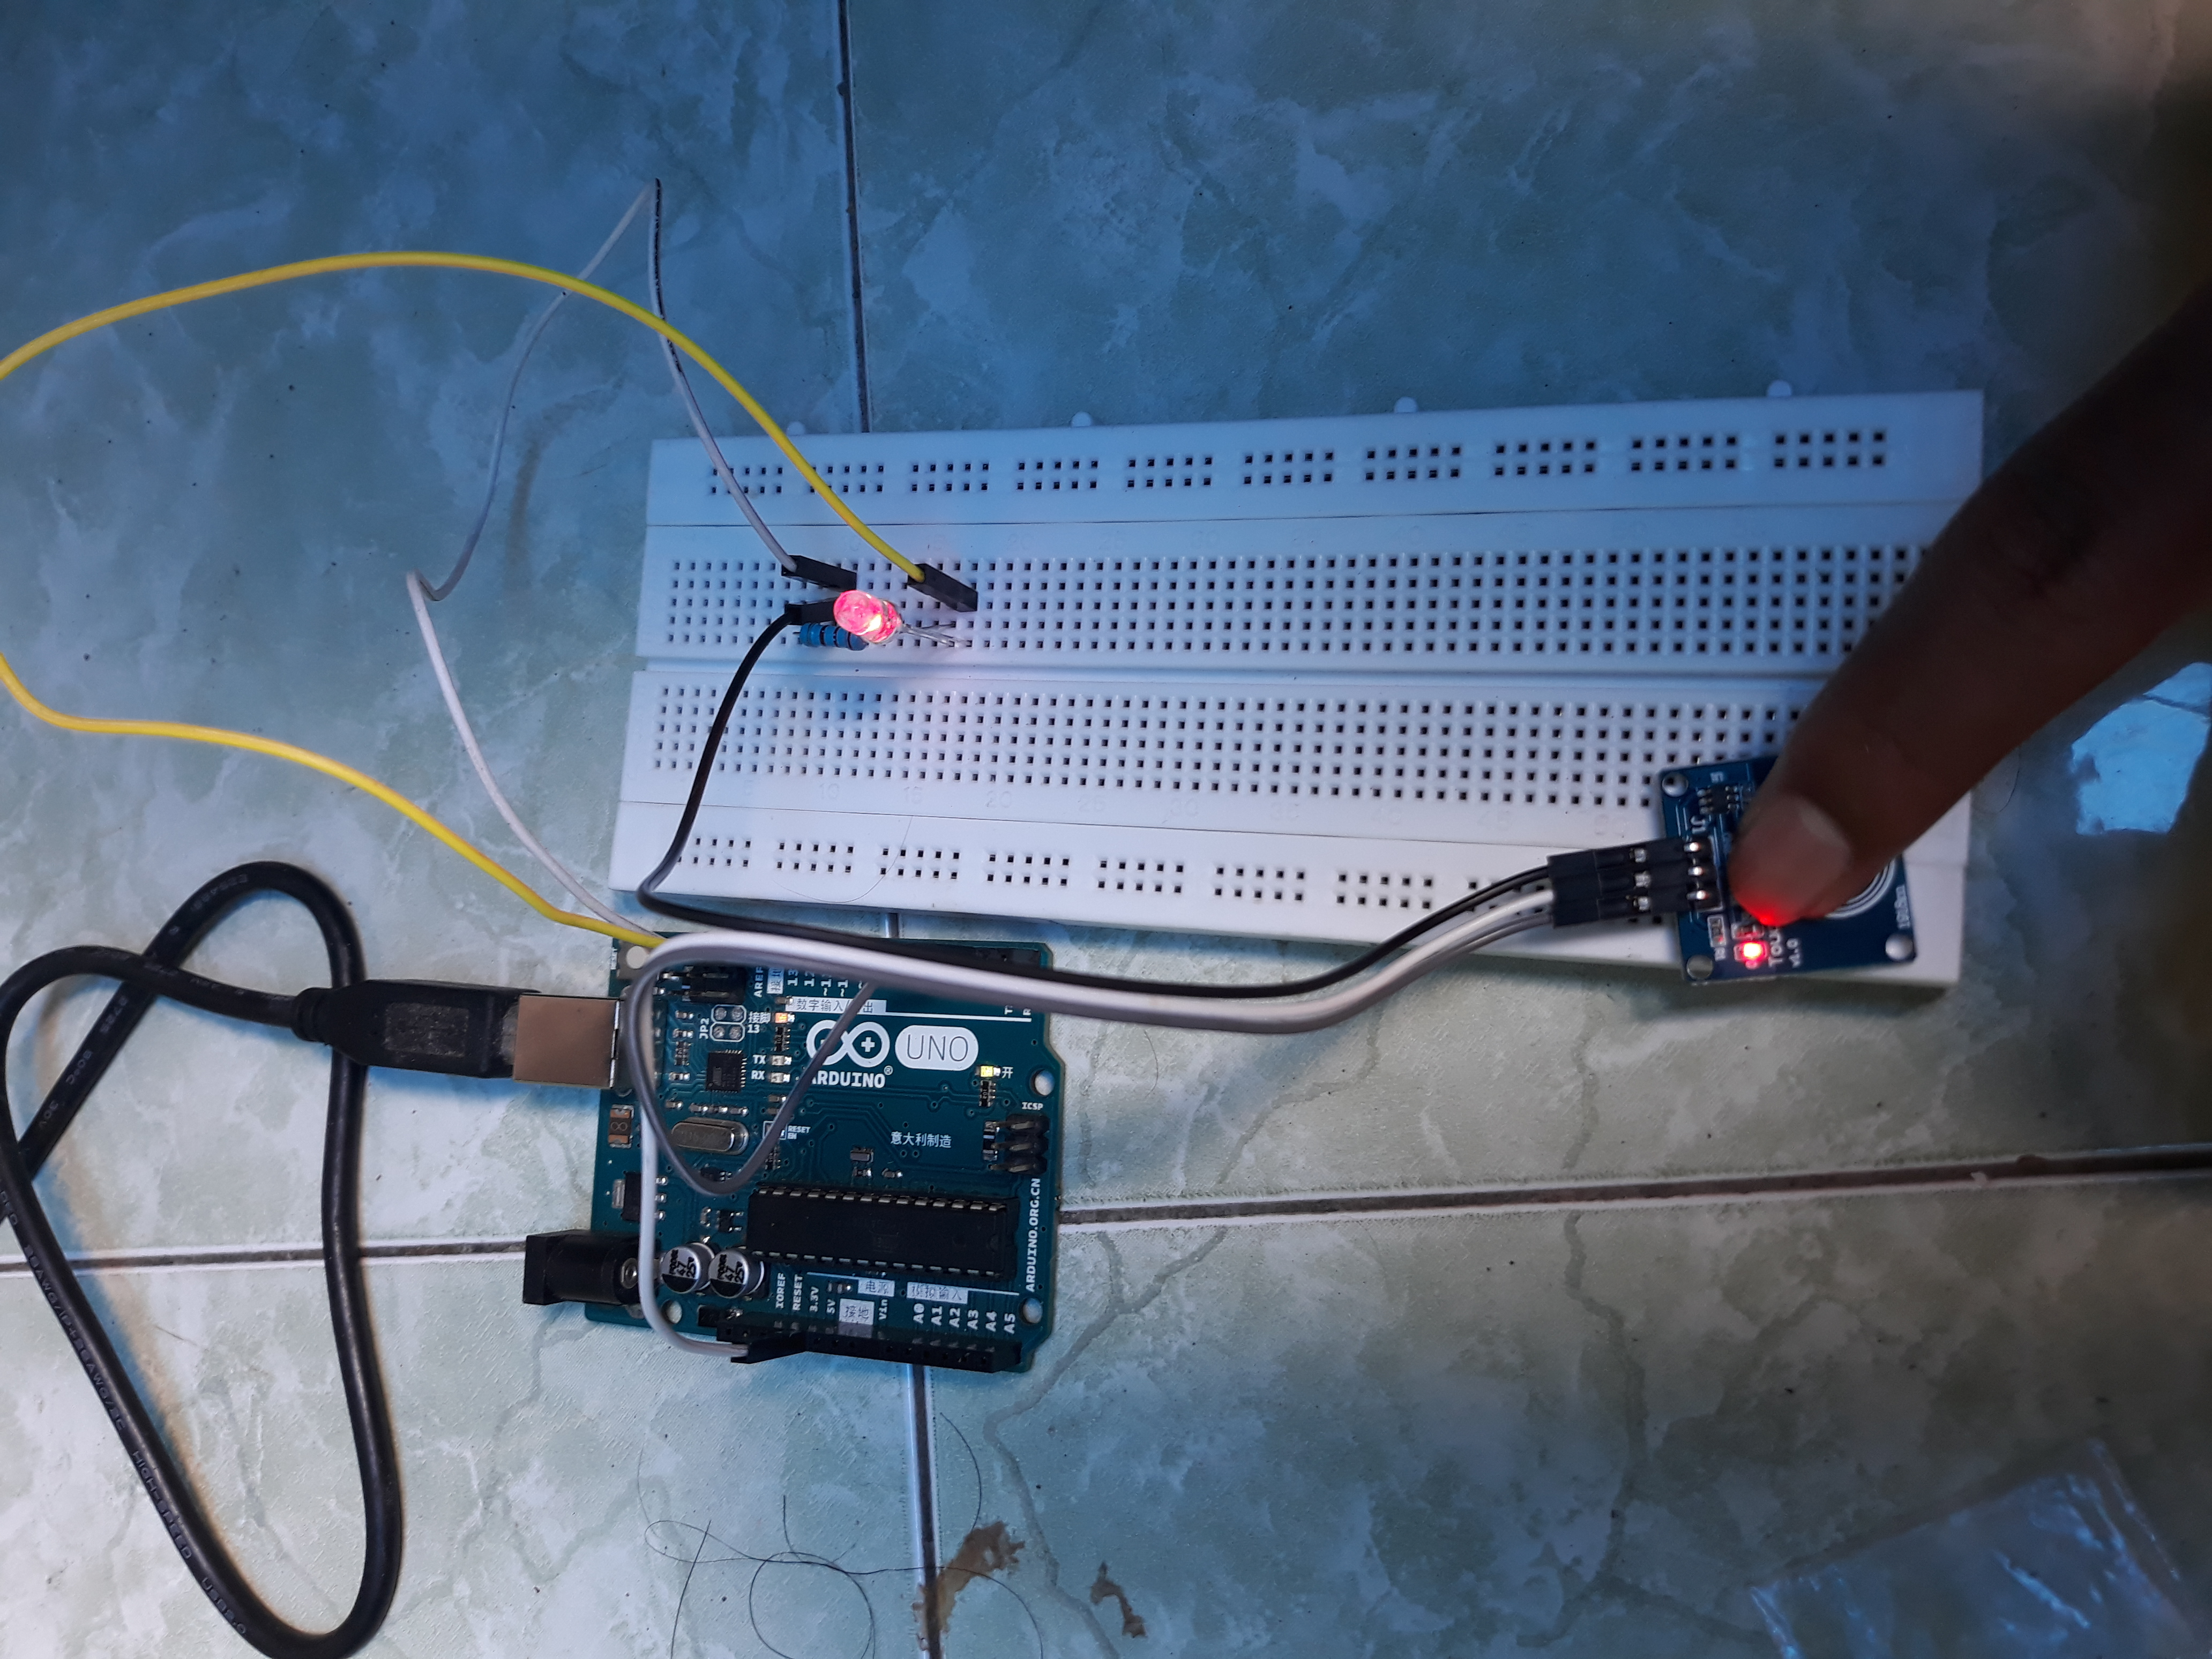
\includegraphics[width=0.5\textwidth]{figures/sesudah.jpg}}
			\caption{Test Sensor}
			\label{sesudah}
			\end{figure}
		
		\begin{figure}[ht]
			\centerline{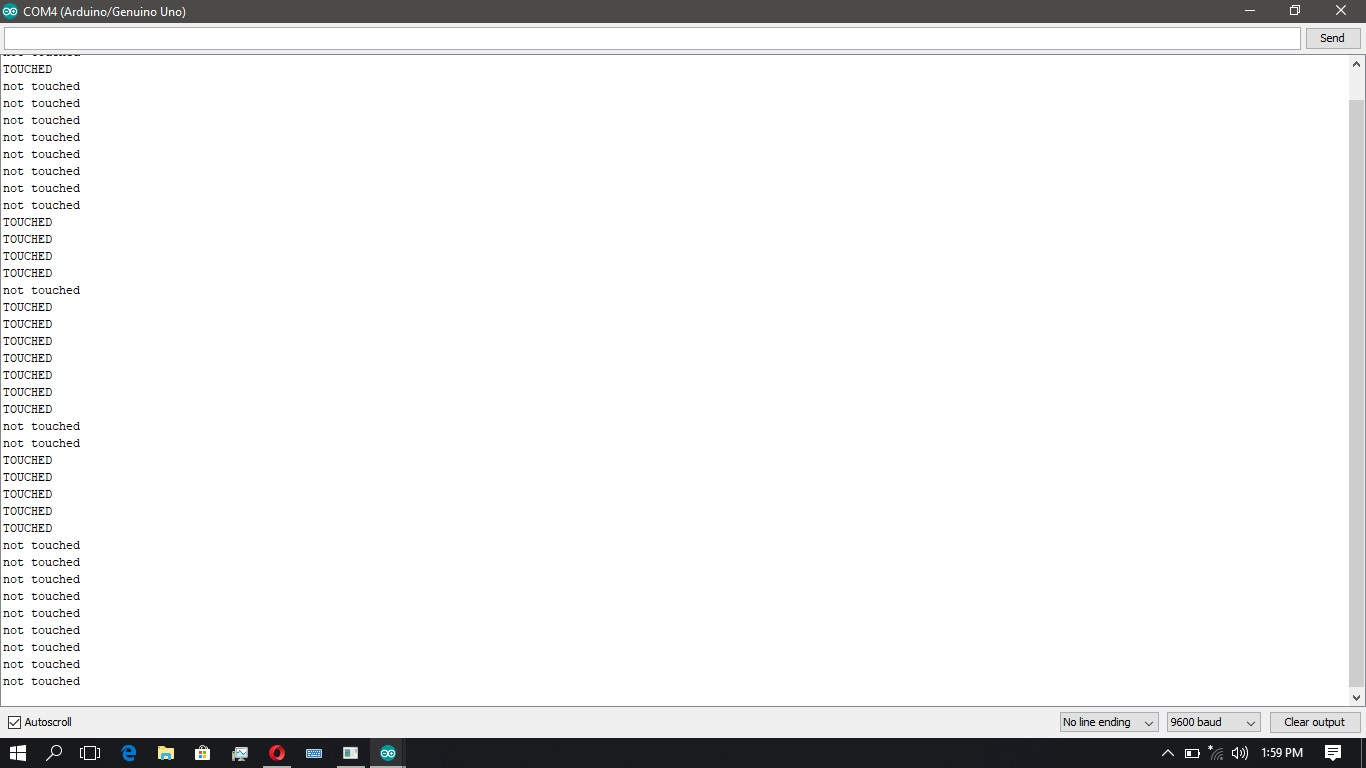
\includegraphics[width=0.5\textwidth]{figures/serialmonitorgua.jpg}}
			\caption{Serial Monitor}
			\label{serialmonitorgua}
			\end{figure}
			
	\ref{sebelum}
	\ref{sesudah}
	\ref{serialmonitor}
	
	\cite{olberding2013cuttable}
